\begin{frame}{What is the HSI Model?}
    The HSI model is a \textbf{statistical} approach to \textbf{anomaly} detection.  HSI does not learn weights through training for later use during inference. 

    \hfill
    
    The model was selected for its use of edge and vertex weighted \textbf{graphs} to obtain relations between data points at different topological and \textbf{temporal scales} by evolving the affinity matrix. 

    \hfill   
    
    HSI was adapted from the paper: \textit{Graph Evolution-Based Vertex Extraction for Hyperspectral Anomaly Detection by Xianchang Yang et al.}
    \hfill
\end{frame}




% \section{What Does HSI Do?}
% \begin{frame}{Model Pipeline}
% \begin{columns}
% \begin{column}{.45\linewidth}
% \begin{itemize}
%     \item Pre-processing
%     \begin{itemize}
%         \item TFIDF IP by quads
%         \item Select Modeling Components with PVA
%     \end{itemize}
    
%     \item Model
%     \begin{itemize}
%         \item \alert<2>{Edge} and \alert<3>{Vertex} Weight Generation
%         \item \alert<4>{Affinity} and \alert<4>{other Graphs} 
%         \item Graph Evolution
%         \item \alert<5>{Penalized Objective Function}
%     \end{itemize}
    
%     \item Inference
%     \begin{itemize}
%         \item Data Selection
%         \item Behavior Exclusion
%         \item Multifilter
%     \end{itemize}
% \end{itemize}
% \end{column}
% \begin{column}{.55\linewidth}\hfill\vfill
% \alert<2>{ $\gamma_i=\sum_{i\neq j}e^{-\left( d_{ij}/d_c\right)^2} \,:\,\vec{\gamma}\in \mathbb{R}^n $ }\\\hfill\vfill
% \alert<3>{$s_{ij}=e^{\left(- d_{ij}/d_c^2 \right)}\,:\, \vec{S}\in \mathbb{R}^{n,n}$}\\\hfill\vfill
% \alert<4>{$ d_{i=j}=\left(\sum_j^n s_{ij}\right)^{-\frac{1}{2}} , d_{i\neq j}=0\,:\, \vec{D}\in \mathbb{R}^{n,n}$\\\hfill\vfill
% $\vec{A}=\vec{\Gamma}\tilde{S}\vec{\Gamma} \,:\, \vec{A}\in \mathbb{R}^{n,n}$\\
% }\hfill\vfill
% \alert<5>{$ f\left(\vec{m}\right)=\frac{1}{2}\vec{m}^T\vec{A}^k\vec{m}+\left(\vec{\gamma}^T\vec{D}\right)^T\vec{m} $}\hfill\vfill
% \end{column}
% \end{columns}


% \end{frame}

% \begin{frame}{Model Pipeline}\vspace{-.25in}
% \begin{columns}
% \begin{column}{.45\linewidth}
% \begin{itemize}
%     \item Pre-processing
%     \begin{itemize}
%         \item TFIDF IP by quads
%         \item Select Modeling Components with PVA
%     \end{itemize}
    
%     \item Model
%     \begin{itemize}
%         \item Edge and Vertex Weight Generation
%         \item Affinity and other Graphs 
%         \item Graph Evolution
%         \item Penalized Objective Function
%     \end{itemize}
    
%     \item Inference
%     \begin{itemize}
%         \item Data Selection
%         \item Behavior Exclusion
%         \item Multifilter
%     \end{itemize}
% \end{itemize}
% \end{column}
% \begin{column}{.55\linewidth}\vspace{-.5in}\bc
% 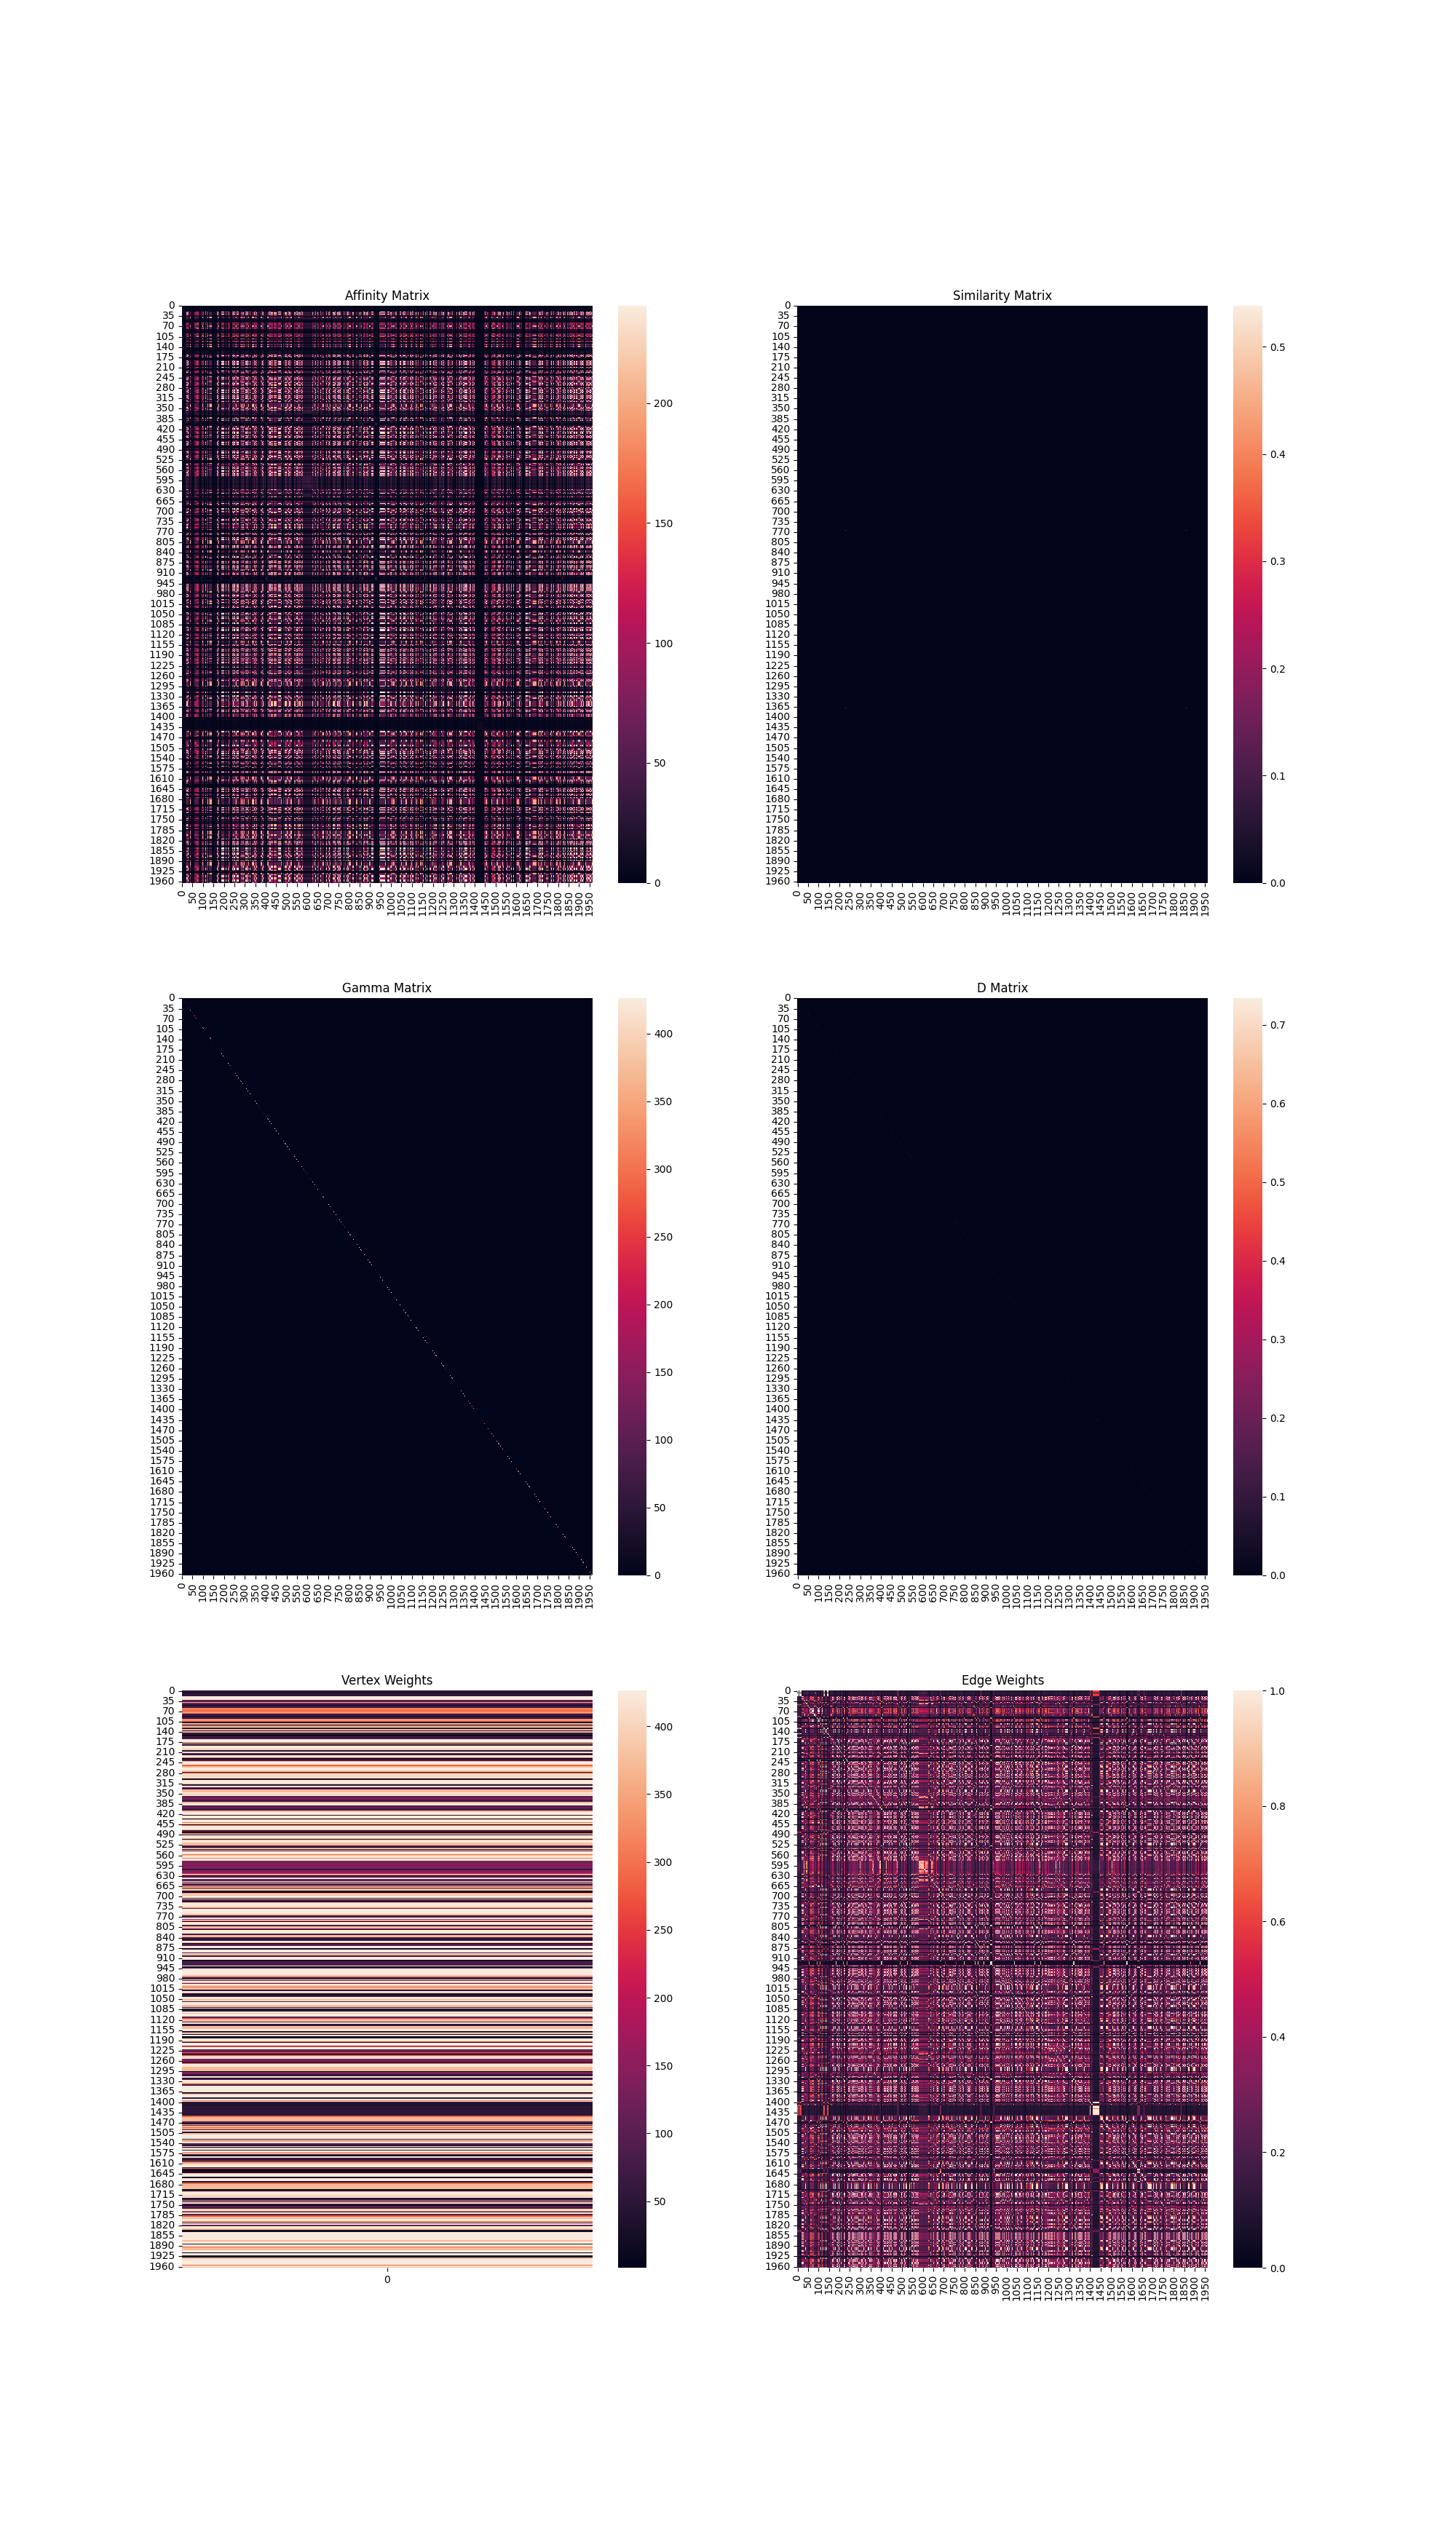
\includegraphics[clip=true, trim=2in 3.25in 2in 3.25in, height=.9\textheight, width=\textwidth ]{../Images/cb_protection_custom_model_weights.png}
% \ec\end{column}
% \end{columns}
% \end{frame}


